\newif\ifglobal

%%%%%%%%%%%%%%%%%%%%%%%
%%% Compile to view %%%
%%%%%%%%%%%%%%%%%%%%%%%

%%%%%%%%%%%%%%%%%%%%%%%%%%%%%%%%%%%%%%%%%%%%%%%%%%%
%%% Readme:                                     %%%
%%% https://www.overleaf.com/read/bwdjvfjksvjy/ %%%
%%%%%%%%%%%%%%%%%%%%%%%%%%%%%%%%%%%%%%%%%%%%%%%%%%%

% >>> M?: marks a module setting number or important notice

% >>> M4: Set {./relative-path} to external files for this module <<<
\def \modulefiles {./26-SDIOSLAVE}
% To add an external file, use:
% (Replace '---' with actual filename)
% '\input{\modulefiles/tables/---.tex}' for tables
% '\includegraphics{\modulefiles/figures/---}' for figures
% '\subfile{\modulefiles/---}' for register files

% >>> M1: This module is in global project? <<<
% 'YES' - uncomment; 'NO' - comment out
\globaltrue

\ifglobal
    \documentclass[main\_\_EN.tex]{subfiles}

\else
    \documentclass[openany, 10pt]{book}

    % >>> M2: In ./00-shared/preamble-trm-module, also find
    %         settings for visibility of todo notes, watermark <<<
    \usepackage{preamble-trm-module}

    % >>> M3: Temporary labels in English,
    %         you can add your own labels there <<<
    \myexternaldocument{./00-shared/temp-labels-en}

\fi %\ifglobal


\setcounter{secnumdepth}{4}


% >>> M5: If this module needs any updates in
% './00-shared/preamble-trm-module.sty'
% (include additional package, etc.), contact your module PM
% or create the file './00-shared/changelog.tex' make the
% necessary updates yourself and document them in this file <<<

% Make text left-aligned and allow latex to break pages naturally, comment out for full justification
\raggedright
\raggedbottom


\begin{document}


% Sets language into which pre-defined bits of text are translated
\selectlanguage{english}
\setenglishformatting

% Do not delete this block
\ifglobal
% Add the following front matter if
% this module is outside of global project
\else
    \InputIfFileExists{readme}{}{}
    \listoftodos
    {\let\clearpage\relax \listofdonetodos}
    \tableofcontents
    %\listoftables
    %\listoffigures
\fi


%%%%%%%%%%%%%%%%%%%%%%%%%
%%% TRM Module Begins %%%
%%%%%%%%%%%%%%%%%%%%%%%%%

\hypertarget{sdioslave}{}
\chapter{SDIO Slave Controller (SDIO)}
\label{mod:sdioslave}

\section{Overview}

The ESP32 features hardware support for the industry-standard Secure Digital (SD) device interface that conforms to the SD Input/Output (SDIO) Specification Version 2.0. This allows a host controller to access the ESP32 via an SDIO bus protocol, enabling high-speed data transfer.

The SDIO interface may be used to read ESP32 SDIO registers directly and access shared memory via Direct Memory Access (DMA), thus reducing processing overhead while maintaining high performance.

 \section{Features}
 \begin{itemize}
    \item Meets SDIO V2.0 specification
    \item Supports SDIO SPI, 1-bit, and 4-bit transfer modes
    \item Full host clock range of 0 \verb+~+ 50 MHz
    \item Configurable sample and drive clock edge
    \item Integrated, SDIO-accessible registers for information interaction
    \item Supports SDIO interrupt mechanism
    \item Automatic data padding
    \item Block size of up to 512 bytes
    \item Interrupt vector between Host and Slave for bidirectional interrupt
    \item Supports DMA for data transfer
\end{itemize}

\section{Functional Description}
\subsection{SDIO Slave Block Diagram}
The functional block diagram of the SDIO slave module is shown in Figure \ref{figure:SDIO Slave block diagram}.

 \begin{figure}[H]
    \centering
    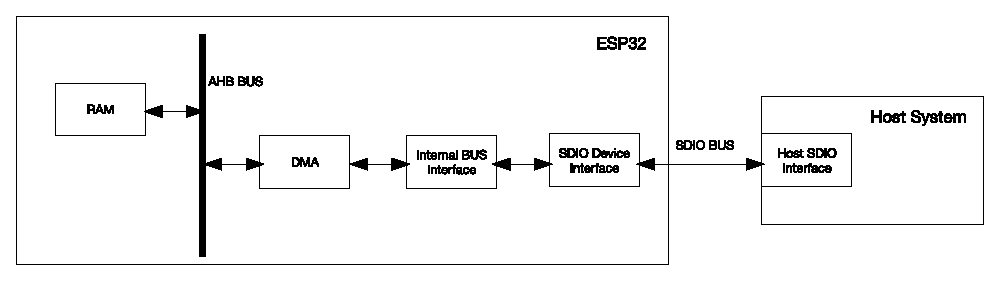
\includegraphics[width=0.7\textwidth]{./26-SDIOSLAVE/figures/SDIOSlaveBlockDiagram}
    \caption{SDIO Slave Block Diagram}
    \label{figure:SDIO Slave block diagram}
\end{figure}

The Host System represents any SDIO specification V2.0-compatible host device. The Host System interacts with the ESP32 (configured as the SDIO slave) via the standard SDIO bus implementation.

The SDIO Device Interface block enables effective communication with the external Host by directly providing SDIO interface registers and enabling DMA operation for high-speed data transfer over the Advanced High-performance Bus (AHB) without engaging the CPU.

\subsection{Sending and Receiving Data on SDIO Bus}

Data is transmitted between Host and Slave through the SDIO bus I/O Function1. After the Host enables the I/O Function1 in the Slave, according to the SDIO protocol, data transmission will begin.

ESP32 segregates data into packets sent to/from the Host. To achieve high bus utilization and data transfer rates, we recommend the single block transmission mode. For detailed information on this mode, please refer to the SDIO V2.0 protocol specification. When Host and Slave exchange data as blocks on the SDIO bus, the Slave automatically pads data-when sending data out-and automatically strips padding data from the incoming data block.

Whether the Slave pads or discards the data depends on the data address on the SDIO bus. When the data address is equal to, or greater than, 0x1F800, the Slave will start padding or discarding data. Therefore, the starting data address should be 0x1F800 - Packet\_length, where Packet\_length is measured in bytes. Data flow on the SDIO bus is shown in Figure \ref{figure:SDIO_BUS_Packet_tran}.

 \begin{figure}[H]
    \centering
    \fbox{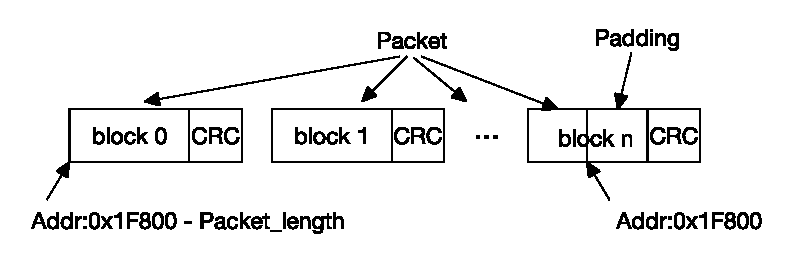
\includegraphics[width=0.65\textwidth]{./26-SDIOSLAVE/figures/SDIO_BUS_Packet_tran.eps}}
    \caption{SDIO Bus Packet Transmission}
    \label{figure:SDIO_BUS_Packet_tran}
\end{figure}

The standard IO\_RW\_EXTENDED (CMD53) command is used to initiate a packet transfer of an arbitrary length. The content of the CMD53 command used in data transmission is as illustrated in Figure
\ref{figure:CMD53 content} below. For detailed information on CMD53, please refer to the SDIO protocol specifications.

 \begin{figure}[H]
    \centering
    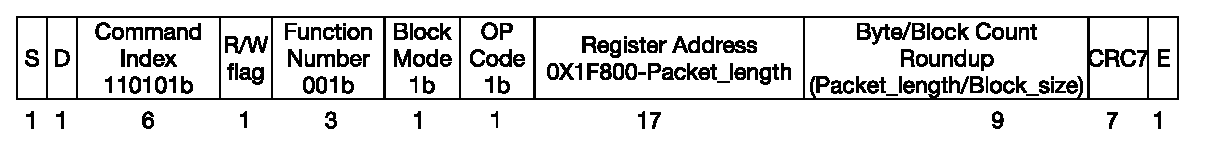
\includegraphics[width=0.9\textwidth]{./26-SDIOSLAVE/figures/CMD53_Content.eps}
    \caption{CMD53 Content}
    \label{figure:CMD53 content}
\end{figure}

\subsection{Register Access}

For effective interaction between Host and Slave, the Host can access certain registers in the Slave via the SDIO bus I/O Function1. These registers are in continuous address fields from \hyperref[regdesc:SLC0HOSTTOKENRDATA]{SLC0HOST\_TOKEN\_RDATA} to S\hyperref[regdesc:SLC0HOSTINTSTREG]{SLC0HOST\_INT\_ST\_REG}.  The Host device can access these registers by simply setting the register addresses of CMD52 or CMD53 to the low 10 bits of the corresponding register address.
The Host can access several consecutive registers at one go with CMD53, thus achieving a higher effective transfer rate.

There are 52 bytes of field between SLCHOST\_CONF\_W0\_REG and SLCHOST\_CONF\_W15\_REG. Host and Slave can access and change these fields, thus facilitating the information interaction between Host and Slave.

\subsection{DMA}

The SDIO Slave module uses dedicated DMA to access data residing in the RAM. As shown in Figure \ref{figure:SDIO Slave block diagram}, the RAM is accessed over the AHB. DMA accesses RAM through a linked-list descriptor. Every linked list is composed of three words, as shown in Figure \ref{figure:Linked Lists}.

 \begin{figure}[H]
    \centering
    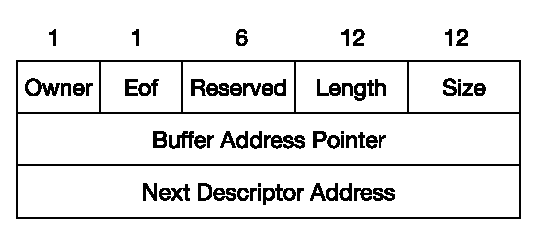
\includegraphics[width=0.5\textwidth]{./26-SDIOSLAVE/figures/Descriptor.eps}
    \caption{SDIO Slave DMA Linked List Structure}
    \label{figure:Linked Lists}
\end{figure}

 \begin{itemize}
    \item Owner: The allowed operator of the buffer that corresponds to the current linked list.
     0: CPU is the allowed operator;
     1: DMA is the allowed operator.
    \item Eof: End-of-file marker, indicating that this linked-list element is the last element of the data packet.
    \item Length: The number of valid bytes in the buffer, i.e., the number of bytes that should be accessed from the buffer for reading/writing.
    \item Size: The maximum number of available buffers.
    \item Buffer Address Pointer: The address of the data buffer as seen by the CPU (according to the RAM address space).
    \item Next Descriptor Address: The address of the next linked-list element in the CPU RAM address space. If the current linked list is the last one, the Eof bit should be 1, and the last descriptor address should be 0.
\end{itemize}

The Slave's linked-list chain is shown in Figure \ref{figure:Linked List}:

 \begin{figure}[H]
    \centering
    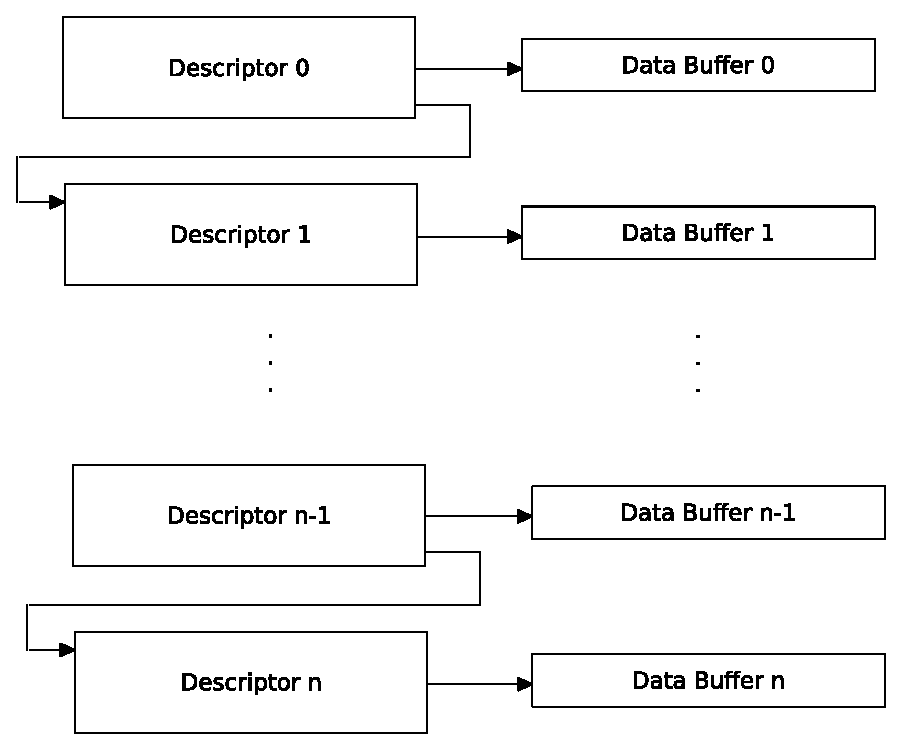
\includegraphics[width=0.55\textwidth]{./26-SDIOSLAVE/figures/Descriptor_chain}
    \caption{SDIO Slave Linked List}
    \label{figure:Linked List}
\end{figure}

\subsection{Packet-Sending/-Receiving Procedure}
The SDIO Host and Slave devices need to follow specific data transfer procedures to successfully exchange data over the SDIO interface.

\subsubsection{Sending Packets to SDIO Host}
The transmission of packets from Slave to Host is initiated by the Slave. The Host will be notified with an interrupt (for detailed information on interrupts, please refer to SDIO protocol). After the Host reads the relevant information from the Slave, it will initiate an SDIO bus transaction accordingly. The whole procedure is illustrated in Figure \ref{figure:Package Sending Procedure}.


 \begin{figure}[H]
    \centering
    \fbox{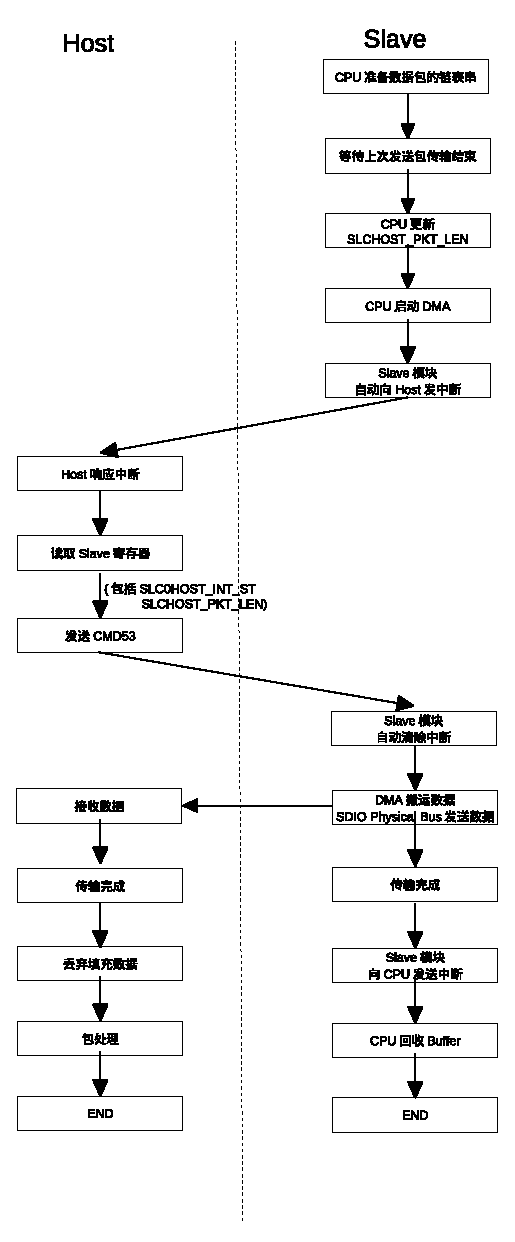
\includegraphics[width=0.4\textwidth]{./26-SDIOSLAVE/figures/Transition_flow.eps}}
    \caption{Packet Sending Procedure (Initiated by Slave)}
    \label{figure:Package Sending Procedure}
\end{figure}

 When the Host is interrupted, it reads relevant information from the Slave by visiting registers SLC0HOST\_INT and SLCHOST\_PKT\_LEN.

\begin{itemize}
    \item SLC0HOST\_INT: Interrupt status register. If the value of SLC0\_RX\_NEW\_PACKET\_INT\_ST is 1, this indicates that the Slave has a packet to send.
    \item SLCHOST\_PKT\_LEN: Packet length accumulator register. The current value minus the value of last time equals the packet length sent this time.
\end{itemize}

In order to start DMA, the CPU needs to write the low 20 bits of the address of the first linked-list element to the SLC0\_RXLINK\_ADDR bit of SLC0RX\_LINK, then set the SLC0\_RXLINK\_START bit of SLC0RX\_LINK.
The DMA will automatically complete the data transfer. Upon completion of the operation, DMA will interrupt the CPU so that the buffer space can be freed or reused.

\subsubsection{Receiving Packets from SDIO Host}
Transmission of packets from Host to Slave is initiated by the Host. The Slave receives data via DMA and stores it in RAM. After transmission is completed, the CPU will be interrupted to process the data. The whole procedure is demonstrated in Figure \ref{figure:Package Receive Procedure}.

 \begin{figure}[H]
    \centering
    \fbox{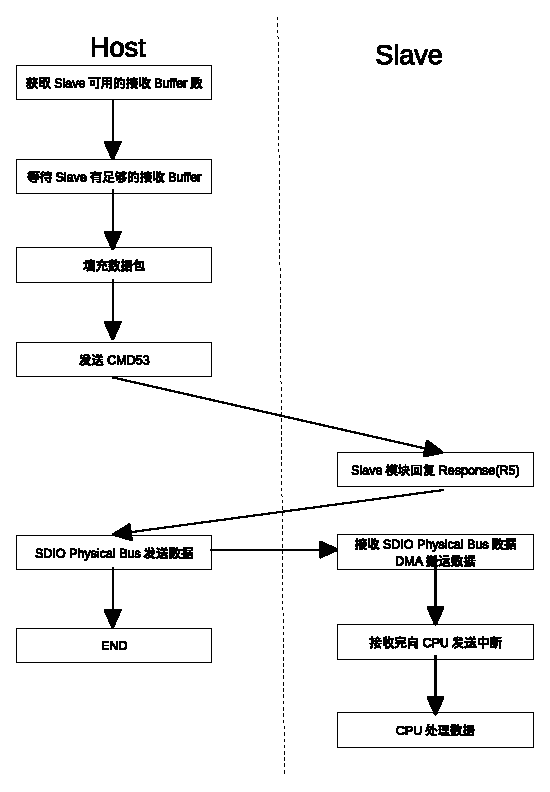
\includegraphics[width=0.45\textwidth]{./26-SDIOSLAVE/figures/Receive_flow.eps}}
    \caption{Packet Receiving Procedure (Initiated by Host)}
    \label{figure:Package Receive Procedure}
\end{figure}


The Host obtains the number of available receiving buffers from the Slave by accessing register SLC0HOST\_TOKEN\_RDATA. The Slave CPU should update this value after the receiving DMA linked list is prepared.

HOSTREG\_SLC0\_TOKEN1 in SLC0HOST\_TOKEN\_RDATA stores the accumulated number of available buffers.

The Host can figure out the available buffer space, using HOSTREG\_SLC0\_TOKEN1 minus the number of buffers already used.

If the buffers are not enough, the Host needs to constantly poll the register until there are enough buffers available.

To ensure sufficient receiving buffers, the Slave CPU must constantly load buffers on the receiving linked list. The process is shown in Figure \ref{figure:Receive load Buffer}.

  \begin{figure}[H]
    \centering
    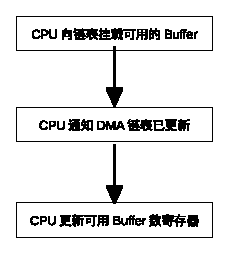
\includegraphics[width=0.3\textwidth]{./26-SDIOSLAVE/figures/Load_Buffer.eps}
    \caption{Loading Receiving Buffer }
    \label{figure:Receive load Buffer}
\end{figure}

The CPU first needs to append new buffer segments at the end of the linked list that is being used by DMA and is available for receiving data.

The CPU then needs to notify the DMA that the linked list has been modified. This can be done by setting bit SLC0\_TXLINK\_RESTART of the SLC0TX\_LINK register. Please note that when the CPU initiates DMA to receive packets for the first time, SLC0\_TXLINK\_RESTART should be set to 1.

Lastly, the CPU refreshes any available buffer information by writing to the SLC0TOKEN1 register.

\subsection{SDIO Bus Timing}\label{SDIO slave timing}
The SDIO bus operates at a very high speed and the PCB trace length usually affects signal integrity by introducing latency. To ensure that the timing characteristics conform to the desired bus timing, the SDIO Slave module supports configuration of input sampling clock edge and output driving clock edge.

When the incoming data changes near the rising edge of the clock, the Slave will perform sampling on the falling edge of the clock, or vice versa, as Figure \ref{figure:Sampling Timing Figure} shows.

 \begin{figure}[H]
    \centering
    \fbox{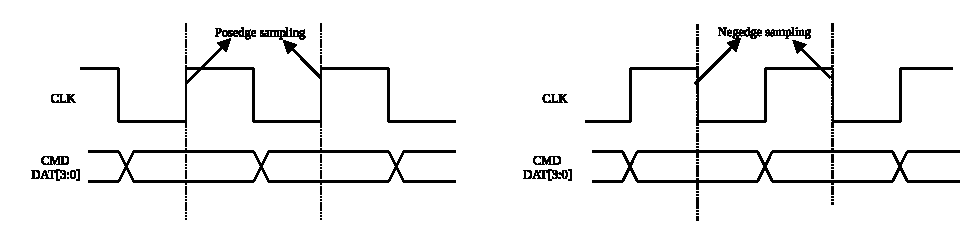
\includegraphics[width=0.8\textwidth]{./26-SDIOSLAVE/figures/Sampling.eps}}
    \caption{Sampling Timing Diagram}
    \label{figure:Sampling Timing Figure}
\end{figure}

By default, the MTDO strapping value determines the Slave's sampling edge. However, users can decide the sampling edge by configuring the \hyperref[regdesc:SLCHOSTCONFREG]{SLCHOST\_CONF\_REG} register, with priority from high to low: (1) Set SLCHOST\_FRC\_POS\_SAMP to sample the corresponding signal at the rising edge; (2) Set SLCHOST\_FRC\_NEG\_SAMP to sample the corresponding signal at the falling edge.

SLCHOST\_FRC\_POS\_SAMP and SLCHOST\_FRC\_NEG\_SAMP fields are five bits wide. The bits correspond to the CMD line and four DATA lines (0-3). Setting a bit causes the corresponding line to be sampled for input at the rising clock edge or falling clock edge.

The Slave can also select which edge to drive the output lines, in order to accommodate for any latency caused by the physical signal path. The output timing is shown in Figure \ref{figure:Output Sequence Figure}.

  \begin{figure}[H]
    \centering
    \fbox{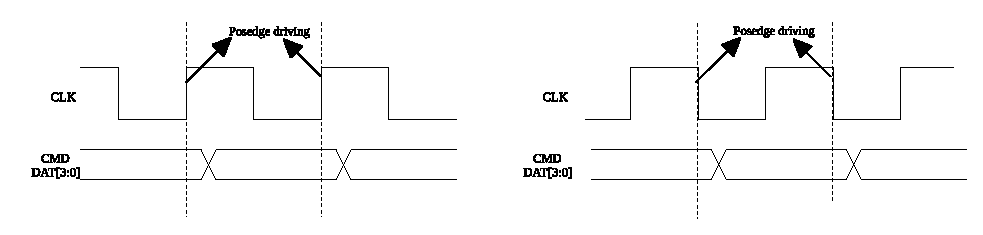
\includegraphics[width=0.8\textwidth]{./26-SDIOSLAVE/figures/Driving.eps}}
    \caption{Output Timing Diagram}
    \label{figure:Output Sequence Figure}
\end{figure}

By default, the GPIO5 strapping value determines the Slave's output driving edge. However, users can decide the output driving edge by configuring the following registers, with priority from high to low: (1) Set SLCHOST\_FRC\_SDIO11 in \hyperref[regdesc:SLCHOSTCONFREG]{SLCHOST\_CONF\_REG} to output the corresponding signal at the falling clock edge; (2) Set SLCHOST\_FRC\_SDIO22 in \hyperref[regdesc:SLCHOSTCONFREG]{SLCHOST\_CONF\_REG} to output the corresponding signal at the rising clock edge; (3) Set HINF\_HIGHSPEED\_ENABLE in \hyperref[regdesc:HINFCFGDATA1REG]{HINF\_CFG\_DATA1\_REG} and SLCHOST\_HSPEED\_CON\_EN in \hyperref[regdesc:SLCHOSTCONFREG]{SLCHOST\_CONF\_REG}, then set the EHS (Enable High-Speed) bit in CCCR at the Host side to output the corresponding signal at the rising clock edge.

SLCHOST\_FRC\_SDIO11 and SLCHOST\_FRC\_SDIO22 fields are five bits wide. The bits correspond to the CMD line and four DATA lines (0-3). Setting a bit causes the corresponding line to output at the rising clock edge or falling clock edge.

{\bfseries Notes on priority setting}: The configuration of strapping pins has the lowest priority when controlling the sampling edge or driving edge. The lower-priority configuration takes effect only when the higher-priority configuration is not set. For example, the MTDO strapping value determines the sampling edge only when SCLHOST\_FRC\_POS\_SAMP and SCLHOST\_FRC\_NEG\_SAMP are not set.

\subsection{Interrupt}
Host and Slave can interrupt each other via the interrupt vector. Both Host and Slave have eight interrupt vectors. The interrupt is enabled by configuring the interrupt vector register (setting the enable bit to 1). The interrupt vector registers can clear themselves automatically, which means one interrupt at a time and no other configuration is required.

\subsubsection{Host Interrupt}
\begin{itemize}
\item {\it SLC0HOST\_SLC0\_RX\_NEW\_PACKET\_INT\label{int:SLC0HOSTSLC0RXNEWPACKETINT}} Slave has a packet to send.
\item {\it SLC0HOST\_SLC0\_TX\_OVF\_INT\label{int:SLC0HOSTSLC0TXOVFINT}} Slave receiving buffer overflow interrupt.
\item {\it SLC0HOST\_SLC0\_RX\_UDF\_INT\label{int:SLC0HOSTSLC0RXUDFINT}} Slave sending buffer underflow interrupt.
\item {\it SLC0HOST\_SLC0\_TOHOST\_BIT\textcolor{red}{\it{n}}\_INT\label{int:SLC0HOSTSLC0TOHOSTBITnINT}} (\textcolor{red}{\it{n}}: 0 \verb+~+ 7) Slave interrupts Host.
\end{itemize}

\subsubsection{Slave Interrupt}
\begin{itemize}
\item {\it SLC0INT\_SLC0\_RX\_DSCR\_ERR\_INT} Slave sending descriptor error.
\item {\it SLC0INT\_SLC0\_TX\_DSCR\_ERR\_INT} Slave receiving descriptor error.
\item {\it SLC0INT\_SLC0\_RX\_EOF\_INT} Slave sending operation is finished.
\item {\it SLC0INT\_SLC0\_RX\_DONE\_INT} A single buffer is sent by Slave.
\item {\it SLC0INT\_SLC0\_TX\_SUC\_EOF\_INT} Slave receiving operation is finished.
\item {\it SLC0INT\_SLC0\_TX\_DONE\_INT} A single buffer is finished during receiving operation.
\item {\it SLC0INT\_SLC0\_TX\_OVF\_INT} Slave receiving buffer overflow interrupt.
\item {\it SLC0INT\_SLC0\_RX\_UDF\_INT} Slave sending buffer underflow interrupt.
\item {\it SLC0INT\_SLC0\_TX\_START\_INT} Slave receiving interrupt initialization.
\item {\it SLC0INT\_SLC0\_RX\_START\_INT} Slave sending interrupt initialization.
\item {\it SLC0INT\_SLC\_FRHOST\_BIT\textcolor{red}{\it{n}}\_INT\label{int:SLC0INTSLCFRHOSTBITnINT}} (\textcolor{red}{\it{n}}: 0 \verb+~+ 7) Host interrupts Slave.
\end{itemize}

\hypertarget{sdioslave-reg-summ}{}
\section{Register Summary}\label{sec:sdioslave-reg-summ}

The addresses in this section are relative to the SDIO Slave base address provided in Table \ref{table:Peripheral_Address_Mapping} in Chapter \ref{mod:sysmem} \textit{\nameref{mod:sysmem}}.

The abbreviations given in Column \textbf{Access} are explained in Section \hyperref[glossary-access-types]{\textit{Access Types for Registers}}.

\subfile{\modulefiles/sdioslave_reg-summary_en}

\clearpage
\section{SLC Registers}

The addresses in this section are relative to the SDIO Slave base address (0x3FF5\_8000) provided in Table \ref{table:Peripheral_Address_Mapping} in Chapter \ref{mod:sysmem} \textit{\nameref{mod:sysmem}}. The absolute register addresses are listed in Section \ref{sec:sdioslave-reg-summ} \textit{\nameref{sec:sdioslave-reg-summ}}. 

For how to program reserved fields, please refer to Section \hyperref[programming-reserved-field]{\textit{Programming Reserved Register Field}}.

\subfile{\modulefiles/slc_reg_en.tex}

\section{SLC Host Registers}

The addresses in this section are relative to the SDIO Slave base address (0x3FF5\_5000) provided in Table \ref{table:Peripheral_Address_Mapping} in Chapter \ref{mod:sysmem} \textit{\nameref{mod:sysmem}}. The absolute register addresses are listed in Section \ref{sec:sdioslave-reg-summ} \textit{\nameref{sec:sdioslave-reg-summ}}. 

For how to program reserved fields, please refer to Section \hyperref[programming-reserved-field]{\textit{Programming Reserved Register Field}}.

\subfile{\modulefiles/host_reg_en.tex}

\section{HINF Registers}

The addresses in this section are relative to the SDIO Slave base address (0x3FF4\_B000) provided in Table \ref{table:Peripheral_Address_Mapping} in Chapter \ref{mod:sysmem} \textit{\nameref{mod:sysmem}}. The absolute register addresses are listed in Section \ref{sec:sdioslave-reg-summ} \textit{\nameref{sec:sdioslave-reg-summ}}. 

For how to program reserved fields, please refer to Section \hyperref[programming-reserved-field]{\textit{Programming Reserved Register Field}}.

\subfile{\modulefiles/hinf_reg_en.tex}

\end{document}
